\begin{frame}
	\frametitle{GWO背景}
	灰狼优化算法(Grey Wolf Optimizer, GWO)是一种模拟灰狼捕食行为的群体智能算法,该算法最先
	由澳大利亚学者 Mirjalili 于 2014 年提出[1],根据灰狼的社会等级将包围、追捕、攻击等捕食任务分配给不
	同等级的灰狼群来完成捕食行为,从而实现全局优化的过程。 GWO 算法具有操作简单、调节参数少、编
	程易实现等特点。在函数优化方面,与其他群智能优化算法相比有明显的优越性。但同时也存在着易陷
	入局部最优、求解精度不高、收敛速度慢等缺点。
\end{frame}


\begin{frame}
	\frametitle{GWO背景}
	\begin{columns}
	\column{.6\textwidth}
		\begin{itemize}
			\item {狼群中的4个等级}
				\begin{itemize}
					\item {$\alpha$: 头狼,狼群的指挥}
					\item {$\beta$: 辅助头狼进行决策}
					\item {$\delta$: 有经验的老狼,警戒/救助}
					\item {$\omega$: 平衡种群内部关系,协助捕猎}
				\end{itemize}
			\item {狼群的3类行为}
				\begin{itemize}
					\item {跟踪, 追逐, 接近猎物}
					\item {追逐, 包围, 骚扰猎物, 直到猎物停止移动}
					\item {向猎物发起攻击}
				\end{itemize}
		\end{itemize}
	\column{.4\textwidth}
		\begin{figure}[htbp]
			\centering
			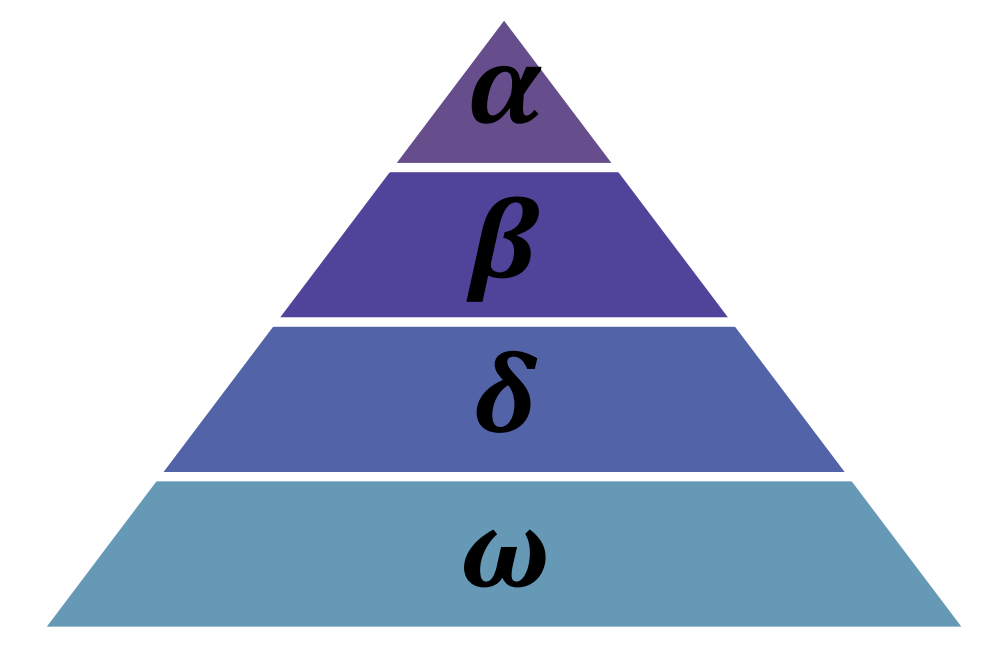
\includegraphics[width=6cm]{pic/wolf1.png}
			\caption{狼群等级结构}
		\end{figure}
	\end{columns}
\end{frame}


\begin{frame}
	\frametitle{GWO背景}
		\begin{figure}[htbp]
			\centering
			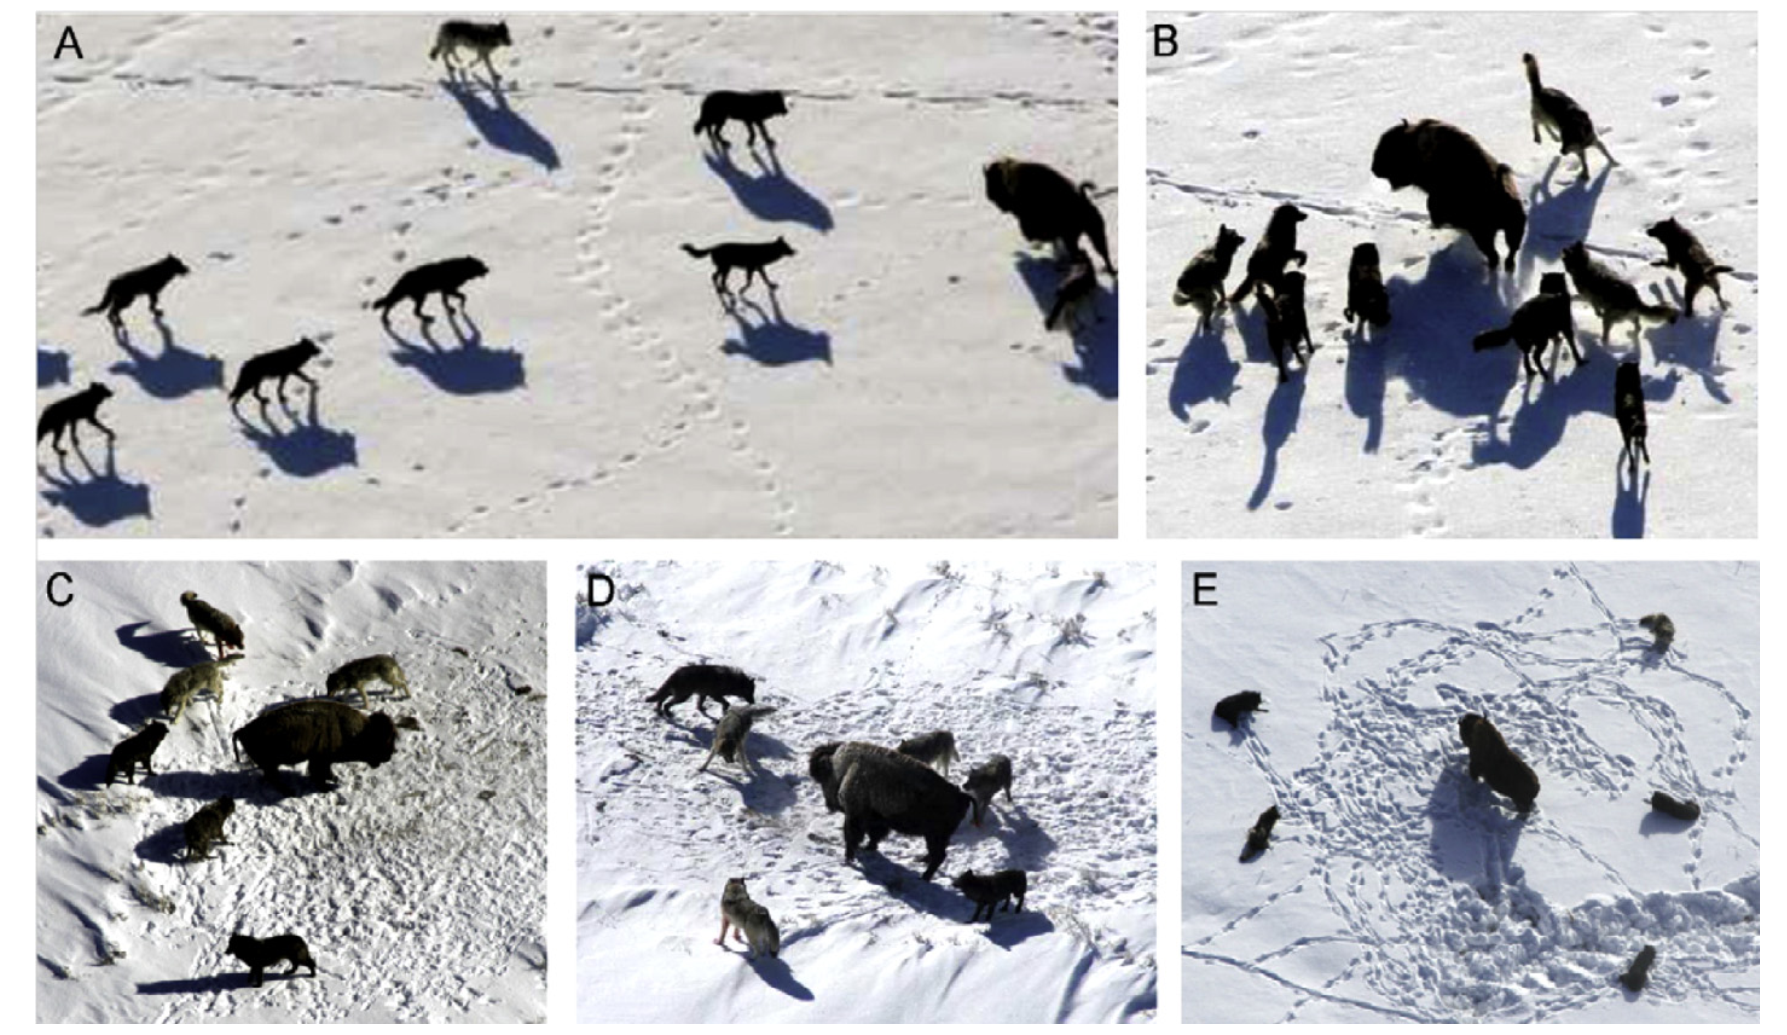
\includegraphics[width=10cm]{pic/wolf2.png}
			\caption{狼群的狩猎行为:A:跟踪猎物;B-D:追逐包围猎物;E:发起攻击}
		\end{figure}
\end{frame}


\begin{frame}
	\frametitle{数学模型——包围/encircling}
	\begin{columns}
	\column{.5\textwidth}
		\begin{equation}
			\vec{D}=|\vec{C} \cdot \vec{X}_{p}(t)-\vec{X}(t)|
		\end{equation}
		\begin{equation}
		\vec{X}(t+1)=\vec{X}(t)-\vec{A}-\vec{D}
		\end{equation}
		其中,$t$代表当前的迭代次数,$\vec{A}$和$\vec{C}$是系数向量,$\vec{X}_p$是当前估计的猎物位置向量,$\vec{X}$是灰狼的位置向量。
		\begin{equation}
			\vec{A}=2\vec{a} \cdot \vec{r}_{1}-\vec{a}
		\end{equation}
		\begin{equation}
		\vec{C}=2 \cdot \vec{r}_2
		\end{equation}
		其中,$\vec{a}$取值在0和2之间,且在迭代过程中逐渐变小,$\vec{r}_1$和$\vec{r}_2$是取值在$[0,1]$之间的随机向量。
	\column{.5\textwidth}
		\begin{figure}[htbp]
			\centering
			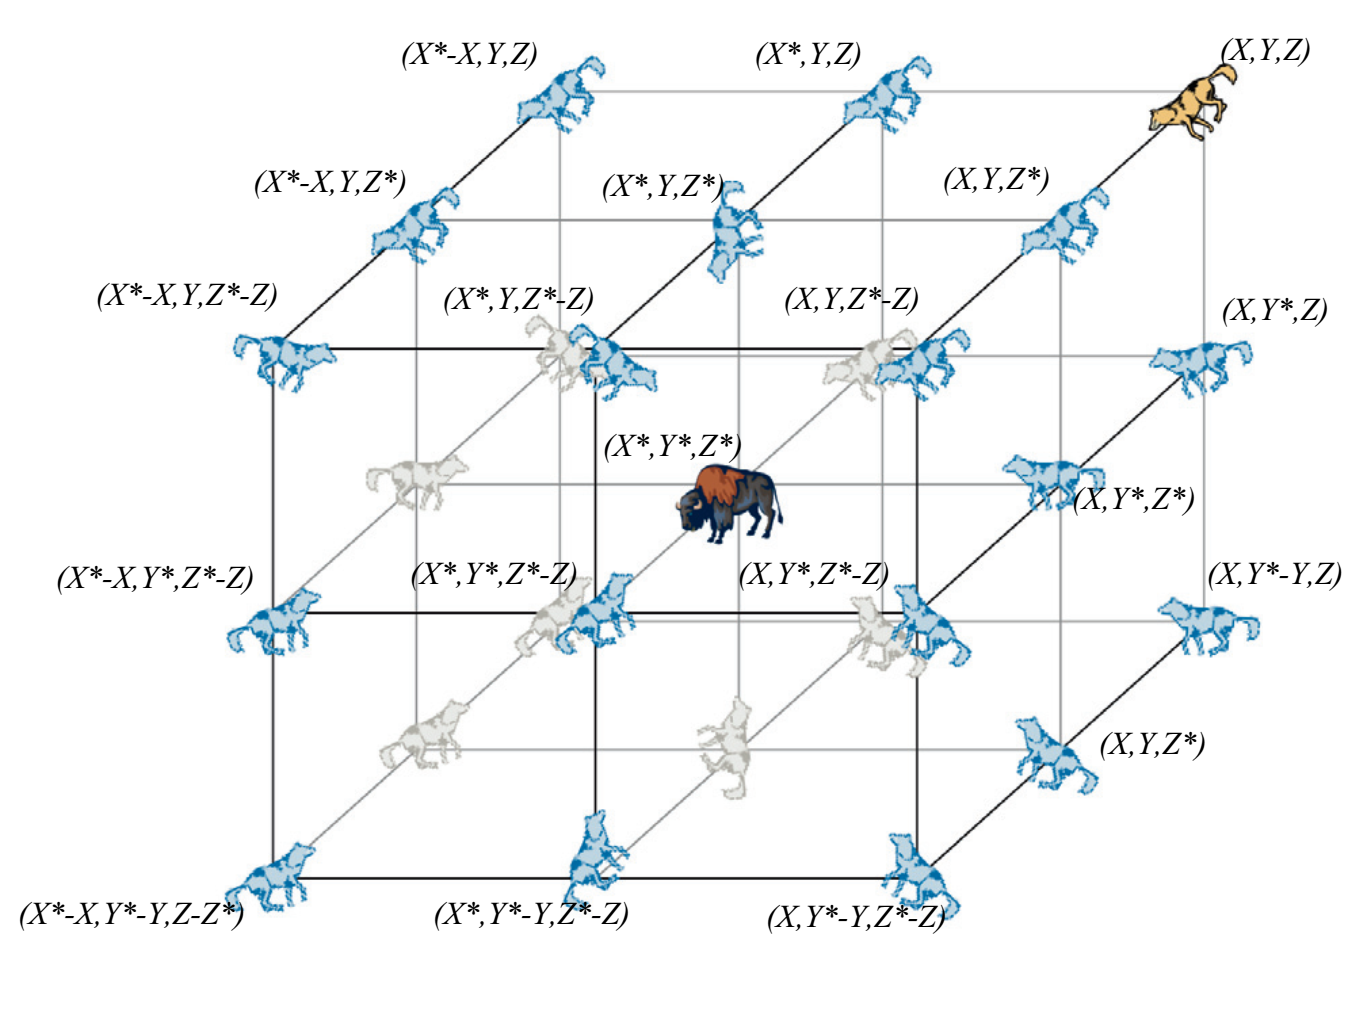
\includegraphics[width=7cm]{pic/wolf3.png}
			\caption{3D空间中灰狼的下一个可能位置}
		\end{figure}
	\end{columns}
\end{frame}


\begin{frame}
	\frametitle{数学模型——捕猎/hunting}
	\begin{itemize}
		\item {实际上,猎物位置$\vec{X}_p$是未知的}
		\item {假设把$\alpha$狼的位置作为最佳候选解,$\beta$和$\delta$次之}
		\item {根据这三个较优解,狼群的每个个体开始进行移动}
	\end{itemize}
	\begin{align}
	&\vec{D}_{\alpha}=|\vec{C}_1 \cdot \vec{X}_{\alpha}-\vec{X}|,\quad \vec{D}_{\beta}=|\vec{C}_2 \cdot \vec{X}_{\beta}-\vec{X}|,\quad \vec{D}_{\delta}=|\vec{C}_3 \cdot \vec{X}_{\delta}-\vec{X}| \\
	&\vec{X}_1=\vec{X}_{\alpha}-\vec{A}_1 \cdot \vec{D}_{\alpha},\quad \vec{X}_2=\vec{X}_{\beta}-\vec{A}_2 \cdot \vec{D}_{\beta},\quad \vec{X}_3=\vec{X}_{\delta}-\vec{A}_3 \cdot \vec{D}_{\delta} \\
	&\vec{X}(t+1)=\cfrac{\vec{X}_1+\vec{X}_2+\vec{X}_3}{3}
	\end{align}
\end{frame}

\begin{frame}
	\frametitle{数学模型——捕猎/hunting}
	\begin{figure}[htbp]
		\centering
		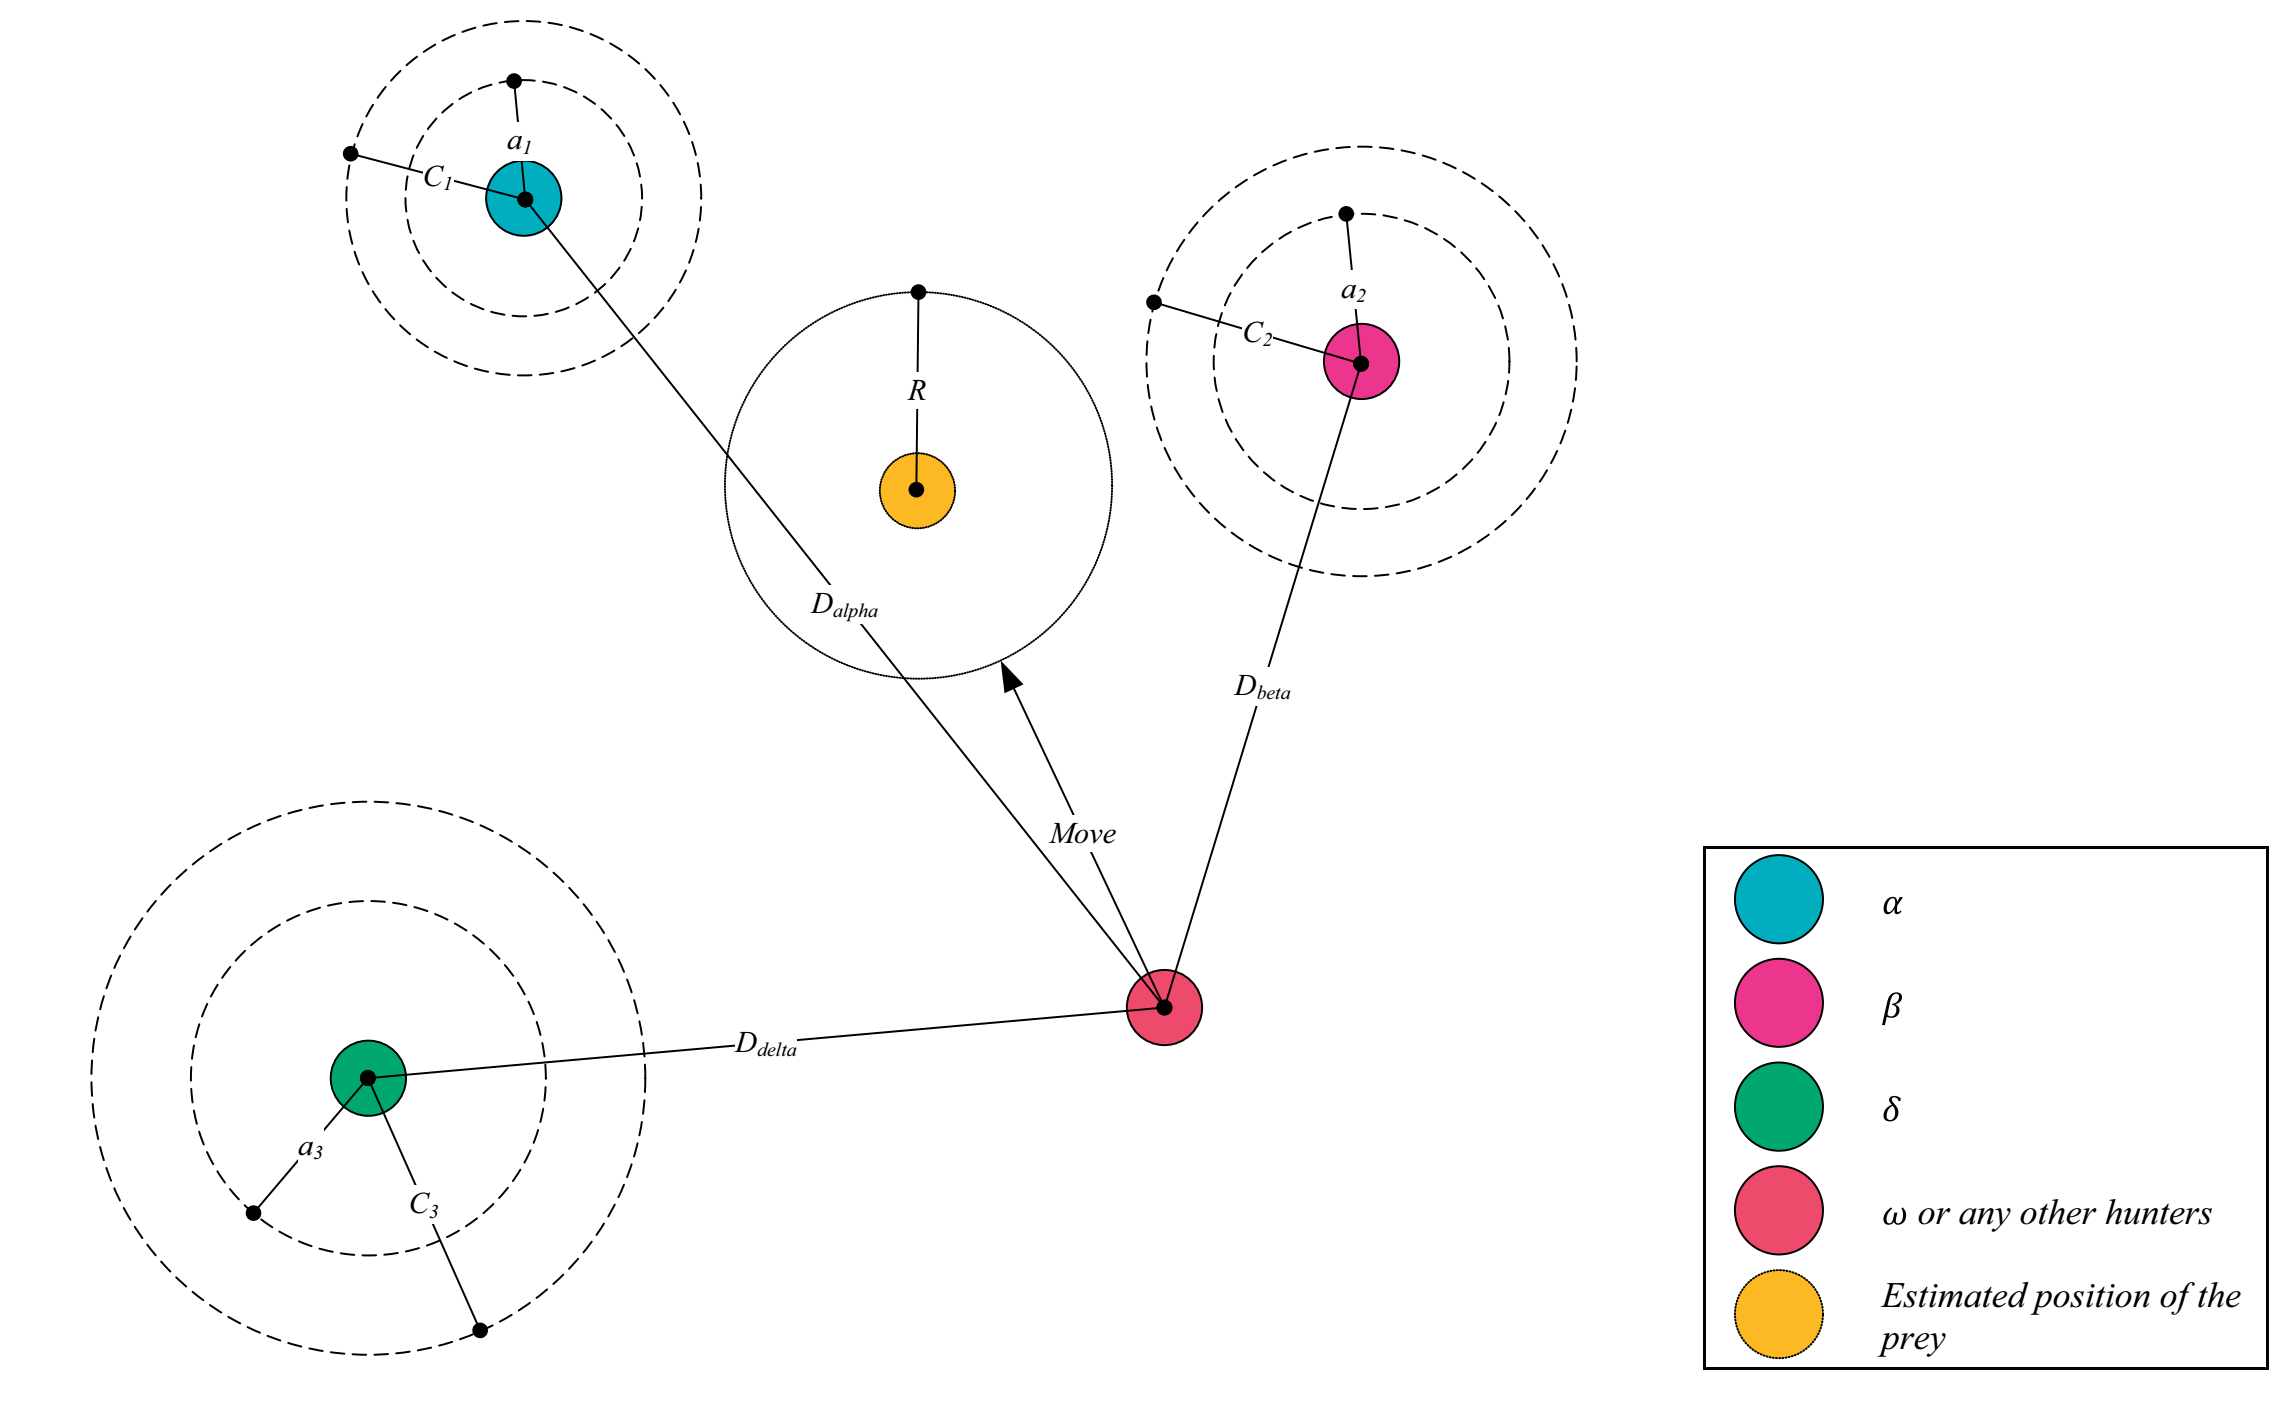
\includegraphics[width=10cm]{pic/wolf4.png}
		\caption{狼群hunting行为示意图}
	\end{figure}
\end{frame}

\begin{frame}
	\frametitle{数学模型——攻击搜寻/attacking,exploration}
	\begin{columns}
	\column{.4\textwidth}
		\begin{itemize}
			\item {Attacking prey (exploitation)}
				\begin{itemize}
					\item {当猎物停止移动时,狼群会发起攻击}
					\item {该过程由a的递减实现,A在[-a,+a]之间变化}
					\item {当|A|<1时,狼群的下一个位置会更加接近猎物位置}
				\end{itemize}
			\item {Search for prey (exploration)}
				\begin{itemize}
					\item {当$|A|>1$时,狼群会远离猎物位置}
					\item {$C$可以看做狼群接近猎物的障碍,它影响了狼和猎物之间距离的衡量,这种游走行为会降低陷入局部最优解的可能性}
				\end{itemize}
		\end{itemize}
	\column{.6\textwidth}
		\begin{figure}[htbp]
			\centering
			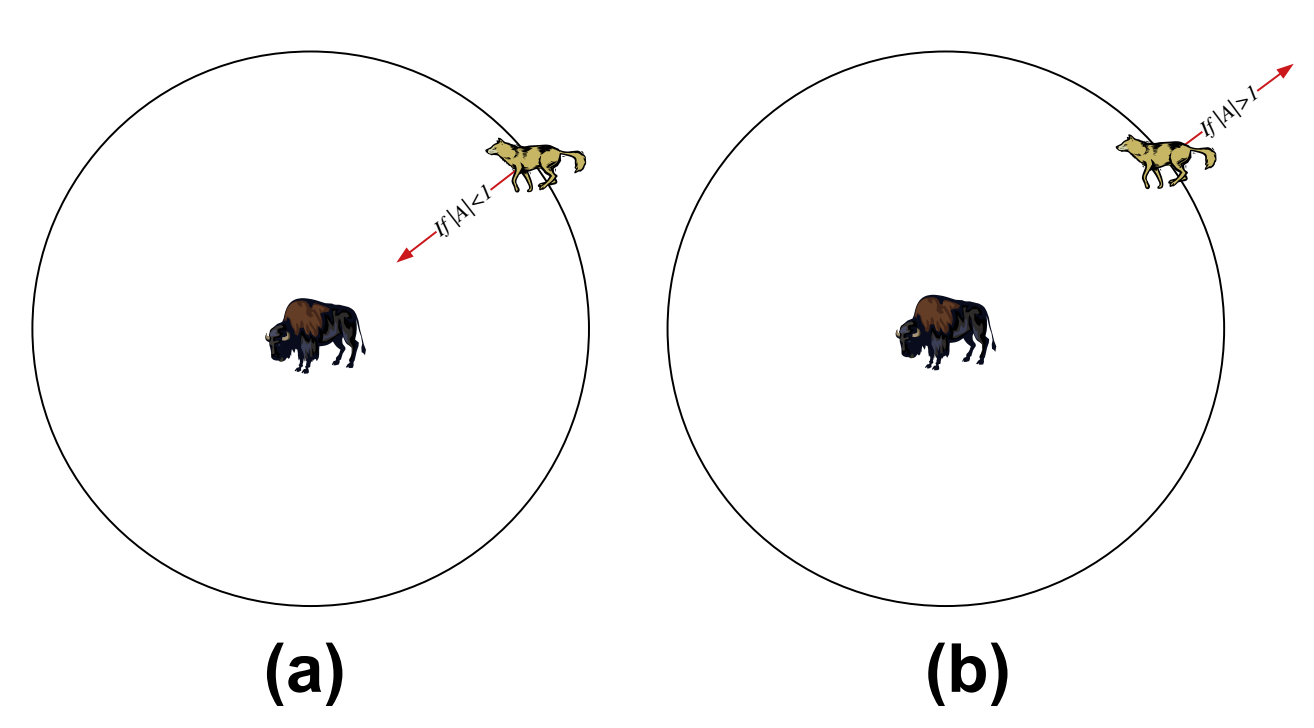
\includegraphics[width=7cm]{pic/wolf5.png}
			\caption{攻击猎物(a)和搜寻猎物(b)}
		\end{figure}
	\end{columns}
\end{frame}


\begin{frame}
	\frametitle{GWO算法}
	\begin{algorithm}[H]
	\caption{GWO}\label{wolf_alg}
	\algsetup{linenosize=\tiny} \scriptsize
		\begin{algorithmic}
			\STATE{Initialize the grey wolf population $X_i(i=1,2,3,...,n)$}
			\STATE{Initialize a, A and C}
			\STATE{Calculate the fitness of each search agent}
			\STATE{$X_{\alpha}$: the best search agent}
			\STATE{$X_{\beta}$: the second best search agent}
			\STATE{$X_{\delta}$: the third best search agent}
			\WHILE{$t < $ Max number of iterations}
				\FOR{each search agent}
					\STATE{Update the position of current search agent}
				\ENDFOR
				\STATE{Update a, A and C}
				\STATE{Caulate the fitness of all aearch agents}
				\STATE{Update $X_{\alpha}$, $X_{\beta}$ and $X_{\delta}$}
				\STATE{$t=t+1$}
			\ENDWHILE
			\STATE{return $X_{\alpha}$}
		\end{algorithmic}
	\end{algorithm}
\end{frame}

\begin{frame}
	\frametitle{Benchmark-unimodal}
	\begin{table}[]
	\centering
	\caption{unimodal functions}
	\label{wolf_table1}
	\begin{tabular}{lccc}
	\hline
	function & dim & range & $f_{min}$ \\ \hline \hline
	$f_1(x)=\sum_{i=1}^{n}x_i^2$ & 30 &  [-100,100]  & 0  \\ \hline
	$f_2(x)=\sum_{i=1}^{n}|x_i|+\prod_{i=1}^{n}|x_i|$ & 30 & [-10,10] & 0 \\ \hline
	$f_3(x)=\sum_{i=1}^{n}(\sum_{j-1}^{i} x_j)^2$ & 30  & [-100,100] &  0 \\ \hline
	$f_4(x)=max_i\{|x_i|,1 \leq i\leq n\}$ & 30 & [-100,100] &  0 \\ \hline
	$f_5(x)=\sum_{i=1}^{n-1}[100(x_{i+1}-x_i^2)^2+(x_i-1)^2]$ & 30 & [-30,30] &  0 \\ \hline
	\end{tabular}
	\end{table}
\end{frame}


\begin{frame}
	\frametitle{Benchmark-multimodal}
	\begin{table}[]
	\centering
	\caption{multimodal functions}
	\label{wolf_table2}
	\begin{tabular}{p{8cm}lccc}  
	\hline
	function & dim & range & $f_{min}$ \\ \hline \hline
	$f_6(x)=\sum_{i=1}^{n} -x_i \sin (\sqrt{|x_i|})$ & 30 &  [-500,500]  & $-418.9829 \times 5$ \\ \hline
	$f_7(x)=\sum_{i=1}^{n}[x_i^2-10\cos (2 \pi x_i)+10]$ & 30 & [-5.12,5.12] & 0 \\ \hline
	$f_8(x)=-20\exp{\left(-0.2\sqrt{\frac{1}{2}\sum_{i=1}^{n}x_i^2}\right)}- \exp{\left(\frac{1}{n}\sum_{i=1}^{n}\cos(2\pi x_i)\right)+20+e}$ & 30  & [-32,32] &  0 \\ \hline
	$f_9(x)=\frac{1}{4000}\sum_{i=1}{n}x_1^2-\prod_{i=1}^{n}\cos\left(\frac{x_1}{\sqrt{i}} \right)+1 $ & 30 & [-600,600] &  0 \\ \hline
	$f_{10}(x)=\frac{\pi}{n}\{10\sin(\pi y_i)+\sum_{i=1}^{n-1}(y_i-1)^2  [1+10{\sin}^2(\pi y_{i+1})]+(y_n-1)^2\}+\sum_{i=1}^{n}u(x_i,10,100,4) $ & 30 & [-50,50] &  0 \\ \hline
	\end{tabular}
	\end{table}
\end{frame}



\begin{frame}
	\frametitle{实验结果}
	\begin{table}[]
	\centering
	\caption{GWO与PSO对比}
	\label{wolf_table3}
	\begin{tabular}{cccccc}
	\multirow{2}{*}{function} & \multirow{2}{*}{min} & \multicolumn{2}{c}{GWO} & \multicolumn{2}{c}{PSO} \\ \cline{3-6} 
	                          &                      & ave        & std        & ave        & std        \\ \hline
	F1                        & 0                    & 6.59e-28   & 6.34e-05   & 1.36e-04   & 2.02e-04   \\
	F2                        & 0                    & 7.18e-17   & 0.029      & 4.21e-02   & 0.045      \\
	F3                        & 0                    & 3.29e-06   & 79.149     & 70.125     & 22.119     \\
	F4                        & 0                    & 5.61e-07   & 1.315      & 1.086      & 0.317      \\
	F5                        & 0                    & 26.81258   & 69.904     & 96.718     & 60.116     \\
	F6                        & -2094.91             & -6123.1    & -4087.44   & -4841.3    & 1152.814   \\
	F7                        & 0                    & 0.310      & 47.356     & 46.704     & 11.629     \\
	F8                        & 0                    & 1.06e-13   & 0.078      & 0.276      & 0.509      \\
	F9                        & 0                    & 0.004      & 0.007      & 0.009      & 0.008      \\
	F10                       & 0                    & 0.053      & 0.020      & 0.007      & 0.026     
	\end{tabular}
	\end{table}
\end{frame}


\begin{frame}
	\frametitle{GWO改进}
	GWO 算法具有操作简单、调节参数少、编程易实现等特点。在函数优化方面,与其他群智能优化算法相比有明显的优越性。但同时也存在着易陷入局部最优、求解精度不高、收敛速度慢等缺点。
	\begin{itemize}
		\item {采用计算分配值的方法提出一种自适应搜索的灰狼求解算法从而加快算法的收敛速度[2]}
		\item {将混沌序列方法引入初始化种群个体,给出了一种寻优性和鲁棒性更好的改进 GWO 算法[3]}
		\item {引入了佳点集理来初始化狼群,并用非固定多段映射罚函数法处理约束条件,利用改进 GWO 算法求解约束优化问题[4]}
	\end{itemize}
	小生境灰狼优化算法(Niche Grey Wolf Optimization, NGWO)[5]利用基本 GWO 算法计算每个灰狼的适应度值。当灰狼距离小于生存半径时,对适应度较差的个体施加惩罚函数,以提高全局搜索能力。
\end{frame}


\begin{frame}
	\frametitle{小生境灰狼算法NGWO}
	\begin{columns}
	\column{.5\textwidth}	
	\begin{itemize}
		\item {“人以类聚,物以群分”}
		\item {将种群划分为多个小生境种群,一小群体为单位进化}
		\item {对小生境种群中适应度较差的个体施加惩罚}
	\end{itemize}
	\column{.5\textwidth}
	个体间距离采用欧氏距离:
	$$d_{ij}=||X_i-X_j||$$
	小生境群体:
	$$d_{ij} < \sigma_{share}$$
	\end{columns}	
\end{frame}


\begin{frame}
	\frametitle{NGWO算法}
	\begin{algorithm}[H]
	\caption{NGWO}\label{nwolf_alg}
	\algsetup{linenosize=\tiny} \scriptsize
		\begin{algorithmic}
			\STATE{Initialize the grey wolf population $X_i(i=1,2,3,...,n)$}
			\STATE{Initialize a, A, C and penatly}
			\STATE{Calculate the fitness $f_i$ of each search agent}
			\STATE{$X_{\alpha}$: the best search agent}
			\STATE{$X_{\beta}$: the second best search agent}
			\STATE{$X_{\delta}$: the third best search agent}
			\WHILE{$t < $ Max number of iterations}
				\FOR{each search agent}
					\STATE{Update the position of current search agent}
				\ENDFOR
				\STATE{Caculate the distance matrix}
				\IF{$d_{ij}<\sigma{share}$}
					\STATE{Set $min\left(f_i,f_j \right)=penalty$}
				\ENDIF
				\STATE{Update a, A and C}
				\STATE{Caulate the fitness of all aearch agents}
				\STATE{Update $X_{\alpha}$, $X_{\beta}$ and $X_{\delta}$}
				\STATE{$t=t+1$}
			\ENDWHILE
			\STATE{return $X_{\alpha}$}
		\end{algorithmic}
	\end{algorithm}
\end{frame}


\begin{frame}
	\frametitle{参考文献}
	\begin{thebibliography}{99} 
	\bibitem{wolf_bib1} Mirjalili, S., Mirjalili, S. and Lewis, A. (2014) Grey Wolf Optimizer. \emph{Advances in Engineering Software}, 69, 46-61
	\bibitem{wolf_bib2} 罗佳, 唐斌. 新型灰狼优化算法在函数优化中的应用[J]. 兰州理工大学学报, 2016, 6(3): 97-101  
	\bibitem{wolf_bib3} 魏政磊, 赵辉, 韩邦杰, 等. 基于自适应 GWO 的多 UCAV 协同攻击目标决策[J]. 计算机工程与应用, 2016, 25(18): 97-101
	\bibitem{wolf_bib4} 龙文, 赵东泉, 等. 求解约束优化问题的改进灰狼优化算法[J]. 计算机应用, 2015, 35(9): 2590-2595
	\bibitem{wolf_bib5} 白媛, 陈京荣, 展之婵. 改进灰狼优化算法的研究与分析[J]. 计算机科学与应用, 2017, 7(6): 562-571
	\end{thebibliography}
\end{frame}